%hw-2.tex
%%%%%%%%%%%%%%%%%%%%%%%%%%%%%%%%%%%%%%%%%%%%%%%%%%%%%%%%%%%%%%%%%%%%%%
%%%%%%            Math 403 Homework \#2, Spring 2025            %%%%%%
%%%%%%                                                          %%%%%%
%%%%%%                 Instructor: Ezra Miller                  %%%%%%
%%%%%%%%%%%%%%%%%%%%%%%%%%%%%%%%%%%%%%%%%%%%%%%%%%%%%%%%%%%%%%%%%%%%%%
\documentclass[11pt]{article}

\oddsidemargin=17pt \evensidemargin=17pt
\headheight=9pt     \topmargin=26pt
\textheight=564pt   \textwidth=433.8pt
\parskip=1ex        %voffset=-6ex

\usepackage{amsmath,amssymb,graphicx,color,enumitem,tikz}%,setspace,mathrsfs}%,hyperref
\setlist[enumerate]{parsep=1.5ex plus 4pt,topsep=0ex plus 4pt,itemsep=0ex}
  \setlist[itemize]{parsep=1.5ex plus 4pt,topsep=-1ex plus 4pt,itemsep=-1.33ex}

\leftmargini=5.5ex
\leftmarginii=3.5ex

%for \marginpar to fit optimally
\hoffset=-1.02in
\setlength\marginparwidth{2.2in}
\setlength\marginparsep{1mm}
\newcommand\red[1]{\marginpar{\linespread{.85}\sf%
		   \vspace{-1.4ex}\footnotesize{\color{red}#1}}}
\newcommand\score[1]{\marginpar{\vspace{-2ex}\color{blue}{#1/3}}\hspace{-1ex}}
\newcommand\extra[1]{\marginpar{\color{blue}{#1/1}}\hspace{-1ex}}
\newcommand\total[2]{\marginpar{\colorbox{yellow}{\huge #1/#2}}}
\newcommand\collab[1]{\marginpar{\vspace{-11ex}\colorbox{yellow}{#1/3}}\hspace{-1ex}}
\newcommand\magenta[1]{\colorbox{magenta}{\!\!#1\!\!}}
\newcommand\yellow[1]{\colorbox{yellow}{\!\!#1\!\!}}
\newcommand\green[1]{\colorbox{green}{\!\!#1\!\!}}
\newcommand\cyan[1]{\colorbox{cyan}{\!\!#1\!\!}}
\newcommand\rmagenta[2][0ex]{\red{\vspace{#1}\magenta{\phantom{:}}\,: #2}}
\newcommand\ryellow[2][0ex]{\red{\vspace{#1}\yellow{\phantom{:}}\,: #2}}
\newcommand\rgreen[2][0ex]{\red{\vspace{#1}\green{\phantom{:}}\,: #2}}
\newcommand\rcyan[2][0ex]{\red{\vspace{#1}\cyan{\phantom{:}}\,: #2}}

%For separated lists with consecutive numbering
\newcounter{separated}

\newcommand{\excise}[1]{}
\newcommand{\comment}[1]{{$\star$\sf\textbf{#1}$\star$}}

%%%%%%%%%%%%%%%%%%%%%%%%%%%%%%%%%%%%%%%%%%%%%%%%%%%
%                                                 %
% TO ENABLE GRADING, DO NOT ALTER ABOVE THIS LINE %
%                                                 %
%%%%%%%%%%%%%%%%%%%%%%%%%%%%%%%%%%%%%%%%%%%%%%%%%%%

%new math symbols taking no arguments
\newcommand\0{\mathbf{0}}
\newcommand\CC{\mathbb{C}}
\newcommand\FF{\mathbb{F}}
\newcommand\NN{\mathbb{N}}
\newcommand\QQ{\mathbb{Q}}
\newcommand\RR{\mathbb{R}}
\newcommand\ZZ{\mathbb{Z}}
\newcommand\bb{\mathbf{b}}
\newcommand\kk{\Bbbk}
\newcommand\mm{\mathfrak{m}}
\newcommand\xx{\mathbf{x}}
\newcommand\yy{\mathbf{y}}
\newcommand\GL{\mathit{GL}}
\newcommand\FL{{\mathcal F}{\ell}_n}
\newcommand\into{\hookrightarrow}
\newcommand\minus{\smallsetminus}
\newcommand\goesto{\rightsquigarrow}

%redefined math symbols taking no arguments
\newcommand\<{\langle}
\renewcommand\>{\rangle}
\renewcommand\iff{\Leftrightarrow}
\renewcommand\implies{\Rightarrow}
\renewcommand\aa{\mathbf{a}}

%to explain about LaTeX commands:
\newcommand\command[1]{\texttt{$\backslash$#1}}

%new math symbols taking arguments
\newcommand\ol[1]{{\overline{#1}}}

%redefined math symbols taking arguments
\renewcommand\mod[1]{\ (\mathrm{mod}\ #1)}

%roman font math operators
\DeclareMathOperator\im{im}

%for easy 2 x 2 matrices
\newcommand\twobytwo[1]{\left[\begin{array}{@{}cc@{}}#1\end{array}\right]}

%for easy column vectors of size 2
\newcommand\tworow[1]{\left[\begin{array}{@{}c@{}}#1\end{array}\right]}


%%%%%%%%%%%%%%%%%%%%%%%%%%%%%%%%%%%%%%%%%%%%%%%%%%%%%%%%%%%%%%%%%%%%%%
\begin{document}%%%%%%%%%%%%%%%%%%%%%%%%%%%%%%%%%%%%%%%%%%%%%%%%%%%%%%
%%%%%%%%%%%%%%%%%%%%%%%%%%%%%%%%%%%%%%%%%%%%%%%%%%%%%%%%%%%%%%%%%%%%%%


\title{\mbox{}\\[-8ex]Math 403 Homework \#2, Spring 2025\\\normalsize
	Instructor: Ezra Miller\\[-2.5ex]}
\author{Solutions by: Thomas Kidane\\[1ex]
Collaborators:Holly Keagan, Ben Greene, Tymon Hendershott, Ricardo Prado Cunha\\
(1 point for each of up to 3 collaborators who also list you)}
\date{Due: 11:59pm Saturday 8 February 2025}

\maketitle

\vspace{-5ex}\collab{3}%

\noindent
\textsc{Reading assignments}\total{36}{45}% cover Lectures 7 - 11
\begin{enumerate}[itemsep=-1ex]\setcounter{enumi}{6}
\item% 7.
for Thu.~30 January
  \begin{itemize}
  \item{}%
  [Serge Lang, \emph{Linear Algebra}, Chapter XII, \S1--\S2]
  separating hyperplanes
  \item{}%
  [Serge Lang, \emph{Linear Algebra}, Chapter XII, \S3--\S4]
  support hyperplane, extreme~point$\!\!$
  \end{itemize}

\item% 8.

for Tue.~4 February
  \begin{itemize}
  \item{}%
  [Wikipedia, \emph{Grassmannian}] as much as you're willing; thru \S3
  (\emph{``as a set''}) at least
  \item{}%
  [Wikipedia, \emph{Group action}] get a feel for the concept; no need
  to overdo it
  \end{itemize}

\item% 9.
for Thu.~6 February
  \begin{itemize}
  \item{}%
  [multivariable calculus, any source]: open \& closed sets;
  differentiability; chain rule \mbox{$D(f \!\circ\! g) = Df \!\circ\!
  Dg$}; inverse function theorem: $Df$ invertible $\implies f$ locally
  invertible%
  \item{}%
  [Wikipedia, \emph{Topological space}] get a feel; through \S5.1
  (\emph{Metric spaces}), say
  \item{}%
  [Wikipedia, \emph{Differentiable manifold}] read up through \S2
  (\emph{Definition})
  \end{itemize}

\item%10.
for Tue.~11 February
  \begin{itemize}
  \item{}%
  [Lax, 7.Isometry, p.87--89] isometry, orthogonal group
  \item{}%
  [Lax, 7.Complex Euclidean structure, p.95--96] unitary matrices
% relevant sections: Adjoint (p.84), Isometry (p.87), Orthogonal Group (p.89)
  \item{}%
  [Treil, \S 5.6--\S 5.7] unitary transformations, rigid motions
  \end{itemize}

\item%11.
for Thu.~13 February
  \begin{itemize}
  \item{}%
  [Treil, \S 6.1--\S 6.2] Spectral theorem, normal operators
  \end{itemize}
\end{enumerate}

\noindent
\textsc{Exercises}% cover Lectures 5 - 8

\begin{enumerate}
\item\ \score{1}%1.
Find the Jordan form of a $5 \times 5$ matrix~$A$ whose sole
eigenvalue is~$3$, given that $A - 3I$, $(A - 3I)^2$, $(A - 3I)^3$,
and $(A - 3I)^4$ have kernels of dimension $2$, $3$, $4$, and~$5$,
respectively.  Do the same thing if the kernel dimensions are $2$,
$4$, $5$, and~$5$, respectively.\red{No explanation.}

\textbf{Solution}

\begin{align}
  \begin{bmatrix}
    3 & 0 & 0 & 0 & 0\\
    0 & 3 & 1 & 0 & 0\\
    0 & 0 & 3 & 1 & 0\\
    0 & 0 & 0 & 3 & 1\\
    0 & 0 & 0 & 0 & 3
  \end{bmatrix}
\end{align}

Upto permuations of jordan blocks.

\begin{align}
  \begin{bmatrix}
    3 & 1 & 0 & 0 & 0\\
    0 & 3 & 1 & 0 & 0\\
    0 & 0 & 3 & 0 & 0\\
    0 & 0 & 0 & 3 & 1\\
    0 & 0 & 0 & 0 & 3
  \end{bmatrix}
\end{align}

Upto permuations of jordan blocks.

\pagebreak



\item\ \score{1}%2.
Find a Jordan form and a corresponding Jordan basis for the matrix \red{Incomplete}
$$%$$ $ 
A =
\left[
\begin{array}{@{}rrrr}
   7\ &\ 1 &  2 &  2 \\
   1\ &\ 4 & -1 & -1 \\
  -2\ &\ 1 &  5 & -1 \\
   1\ &\ 1 &  2 &  8 
\end{array}
\right].
$$%$$ $

\textbf{Solution}

The characteristic polynomial for this matrix is $p(x)=(x-6)^4$. The geometric multiplicity is 2.
Which means that there are 2 jordan blocks. The eigen vectors are.

\begin{align*}
  v_1= \begin{bmatrix}
   -1 \\
    -1 \\
    1 \\
    0
  \end{bmatrix} \\
  v_2 = \begin{bmatrix}
    -1 \\
   -1 \\
    0 \\
    1
  \end{bmatrix}
\end{align*}

The geometric multiplicities are 2,3 and 4 for $(A-6I), (A-6I)^2,$ and $(A-6I)^3$ respectively.
So the matrix's jordan form is as below.

\begin{align}
  \begin{bmatrix}
    6 & 0 & 0 & 0\\
    0 & 6 & 1 & 0\\
    0 & 0 & 6 & 1\\
    0 & 0 & 0 & 6
  \end{bmatrix}
\end{align}


\pagebreak





\item\ \score{3}%3.
Let $V$ be a vector space over~$\RR$ or~$\CC$ of finite dimension.
Let $\varphi: V \into W$ be an injective homomorphism.  Show that if
$\mu$ is a norm on~$W$ then $\mu \circ \varphi$ is a norm on~$V$.


\textbf{Solution}


For $\mu \circ \varphi$ to be a norm on $W$ it has to satisify 
certain properities of a norm.

1. $\mu \circ \varphi(x)=0 \Leftrightarrow x=0$

Since $\mu$ is already a norm,$\mu (x)=0 \Leftrightarrow x=0$, but $\varphi$
is injective therefore $ker(\varphi) = {0}$, so $\mu \circ \varphi(x)=0 \Leftrightarrow x=0$.

2. $\mu \circ \varphi(\alpha x)=|\alpha| \mu \circ \varphi(x)$ for $\alpha \in $ the field.

Since $\mu$ is a norm, then $\mu(\alpha x) = |\alpha| \mu (x)$, and since $\varphi$ is linear $\varphi(\alpha x)=\alpha \varphi (x)$. 
$\mu \circ \varphi(\alpha x)= \mu(\alpha \varphi(x) ) = |\alpha| \mu \circ \varphi(x)$, satisifing the property.

3. $\mu \circ \varphi (x+y)$ $ \leq$ $\mu \circ \varphi (x) + \mu \circ \varphi(y)$
Since $\mu$ is a norm $\mu (x+y) \leq \mu(x) + \mu(y)$. So 
$\mu \circ \varphi (x+y) = \mu (\varphi(x) + \varphi(y)) \leq \mu \circ \varphi(x) + \mu \circ \varphi (y)$.

So $\mu \circ \varphi$ is a norm on $W$.


\pagebreak
\item\ \score{2}%4.
Let $\nu$ be a norm on $V = \RR^n$ or~$\CC^n$ with unit $\nu$-ball
$B_\nu = \{\xx \in V \mid \nu(\xx) \leq 1\}$.  Prove that $B_\nu$ is
closed, bounded, convex, and \emph{equilibrated}: $\xx \in B_\nu$ and
$|\alpha| \leq 1 \implies \alpha\xx \in B_\nu$.  Also show that the
origin lies interior to~$B_\nu$.  Conversely, if $B \subseteq V$ is
closed, bounded, convex, equilibrated subset with $0$ in its interior,
then a norm $\nu_B: V \to \RR$ with unit ball~$B$ can be defined by
$\nu_B(\xx) = \inf\{\alpha > 0 \mid \frac 1\alpha \xx \in B\}$.

\textbf{Solution}


Claim 1: $B_\nu$ is closed, bounded, convex and equilibrated.

Closed:- Assume for the sake of contradiction, that there exist a sequence of
of points inside $B_\nu$ such that it converges to a value $a$, such that $a \notin B_\nu$.
Therefore $\nu(a) > 1$, but since $a$ is a the limit of some sequence
all of whose elements are in $B_\nu$ then $\nu(a) \leq 1$, which contradicts the 
assumption that $a \notin B_\nu$. \red{You need a little more here: pick an open around $a$.}

Bounded:- All points have norm $\leq 1$, and therefore it is bounded.

Convex:- Take any two points,$x,y \in B_\nu$.

All points $\alpha x + (1-\alpha) y, \alpha \in [0,1]$ are in $B_\nu$.
\\
Proof:- Since $\nu(\alpha x + (1-\alpha) y) \leq \alpha \nu(x) + (1-\alpha)\nu(y)$\\

$\nu(x) \leq 1$ and $\nu(y) \leq 1$, so $\alpha \nu(x) + (1-\alpha)\nu(y) \leq \alpha + (1-\alpha) = 1$.

So all points have norm$\leq$ 1, and are therefore in the set. So $B_\nu$ is convex.

Equilibrated: For $|x| \leq 1$, $\alpha x \in B_\nu$.

$\nu(x) \leq 1, \nu(\alpha x)= |\alpha|\nu(x) \leq |\alpha| \leq 1 \Rightarrow \alpha x \in B_\nu$.

Origin lies in the interior: Take the open ball of radies 1/2. This ball is contained inside $B_\nu$, and since 
it is open all the points are in the interior.

Converse claim:- If $B$ is a closed, bounded, convex, equilibrated subset with 0 in its interior then, 
a norm $\nu_{B}$ : $V \rightarrow R^{+}$ with unit ball $B$ can be defined by $\nu_{B}(x)=inf\left\{\alpha \geq 0\; |\; 1/\alpha \in B\right\}$

Property $\#$1: $\nu_{B}(x)=0 \Leftrightarrow x=0$

This is trivially true(atleast by setting $\nu_{B}(0)=0$ in the definition).\red{One direction is obvious, but the other is non-trivial: it used boundedness.}

Property $\#$2: $\nu(\beta x)=|\beta|\nu(x)$

Lemma :- $\nu(x) = \nu(-x)$

Proof:- By equilibration, if $x \in B$, then $-x \in B$ as well.\\
Let $\nu(x) = \alpha_{1}$ and $\nu(-x)=\alpha_2$. If
$\alpha_1 \neq \alpha_2$ then without loss of generalitiy(WLOG) assume $\alpha_1 > \alpha_2$.

$1/\alpha_{2} \; x \in B$, but this also implies $\frac{-1}{\alpha_{2}} \; x \in B$, so 
$\frac{1}{\alpha_2} $-x$ \in B$, but $\alpha_2 < \alpha_1$ and therefore contradiction,
therefore $\alpha_1 = \alpha_2$.

Assume $\nu(\beta x)= \alpha \Leftrightarrow \frac{\beta}{\alpha} x \in B \Leftrightarrow \frac{\beta}{-\alpha} \in B \Rightarrow \frac{\beta}{|\alpha|} \in B$.

Property $\#$ 3: $\nu(x+y) \leq \nu(x) + \nu(y)$\\

$(\frac{1}{\alpha_1 + \alpha_2})(x+y)=(\frac{1}{\alpha_1+\alpha_2})x+(\frac{1}{\alpha_1+\alpha_2})y$.
\\$(\frac{\alpha_1}{\alpha_1+\alpha_2} \frac{1}{\alpha_1})x+(\frac{\alpha_2}{\alpha_1+\alpha_2} \frac{1}{\alpha_2})y$ and since $\frac{\alpha_1}{\alpha_1+\alpha_2} \frac{1}{\alpha_1} x \in B$ and $\frac{\alpha_2}{\alpha_1+\alpha_2} y \frac{1}{\alpha_2} \in B$ then $\frac{\alpha_1}{\alpha_1+\alpha_2} \frac{1}{\alpha_1}x+\frac{\alpha_2}{\alpha_1+\alpha_2} \frac{1}{\alpha_2}y \in B$ because
this is a convex combination of points in $B$, and therefore the norm has to be smaller or equal to $\alpha_1+\alpha_2$.


\pagebreak

\item\ \score{0}%5.
The Hahn--Banach theorem says that for any norm~$\nu$ on~$\CC^n$ and
any subspace $V \subseteq \CC^n$, if $\varphi: V \to \CC$ is a linear
functional whose maximum magnitude $|\varphi(\xx)|$ for $\xx$ in the
unit $\nu$-sphere of~$V$ is~$\alpha$, then $\varphi$ can be extended
to a linear functional on~$\CC^n$ whose maximum magnitude on the unit
$\nu$-sphere in~$\CC^n$ is~$\alpha$.  Show that the Hahn--Banach
theorem is equivalent to the statement that separating hyperplanes
exist for points outside of any closed, bounded, convex, equilibrated
set that contains~$0$ in its interior.

\item\ \score{3}%6.
Let $V$ be the vector space of real (or complex) absolutely convergent
series.  The function $x \mapsto \Vert x \Vert_p =
\big(\sum_{i=1}^\infty |x_i|^p\big){}^{\frac 1p}$ for $p \geq 1$ is a
norm on~$V$.  (You may assume this, although no complaints if you'd
like to prove it.)  Prove that $\Vert x \Vert_p$ is not topologically
equivalent to $\Vert x \Vert_q$ if $p < q$.

\textbf{Solution}

Assume $q>p$. If the two norms are topologically equivalent, then you can find a constant $\alpha$ and $\beta$ such 
that $\alpha \Vert x \Vert_p \leq \Vert x \Vert_q \leq \beta \Vert x \Vert_p$.

Assume that this alpha does exist and is $>0$. We will make a sequence that 
has a sum of 1, and we will see what happens to the ratio when we take the number of
of terms to the limit.

\begin{align*}
  \text{Let } x_i = \frac{1}{n} \text{ for } n \text{ terms and } 0 \text{ otherwise}\\
  \text{Then } \sum_{i=1}^n |x_i|^p = \frac{1}{n^{p-1}} \text{ and } \sum_{i=1}^n |x_i|^q = \frac{1}{n^{q-1}}\\
  \text{Therefore } \frac{\|x\|_q}{\|x\|_p} = \frac{(\frac{1}{n^{q-1}})^{\frac{1}{q}}}{(\frac{1}{n^{p-1}})^{\frac{1}{p}}} = n^{\frac{p-1}{p} - \frac{q-1}{q}}\\
  \text{As } n \to \infty \text{, this ratio approaches } 0 \text{ since } q > p\\
  \text{This contradicts the existence of } \alpha > 0
\end{align*}

\pagebreak

\item\ \score{3}%7.
Sketch the convex hull of \red{Nice use of Tikz}
$\Bigg\{\tworow{1\\2},\tworow{1\\-1},\tworow{1\\3},\tworow{-1\\1}\Bigg\}$
and
$\Bigg\{\tworow{-1\\2},\tworow{2\\3},\tworow{-1\\-1},\tworow{1\\0}\Bigg\}$.

\textbf{Solution}

\begin{center}
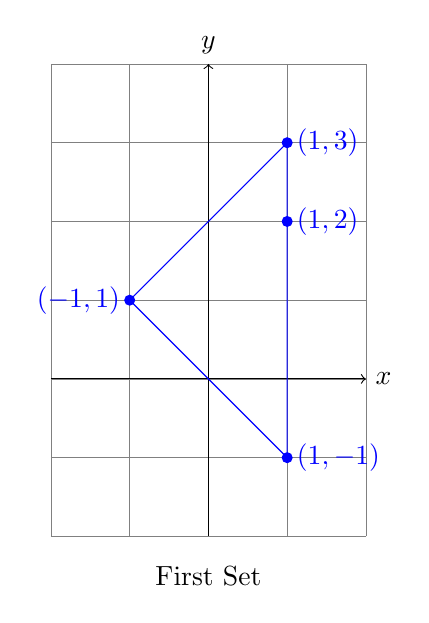
\begin{tikzpicture}[scale=1]
    % Grid and axes for first plot
    \draw[very thin,gray] (-2,-2) grid (2,4);
    \draw[->] (-2,0) -- (2,0) node[right] {$x$};
    \draw[->] (0,-2) -- (0,4) node[above] {$y$};
    
    % Points for first set
    \fill[blue] (1,2) circle (2pt) node[right] {$(1,2)$};
    \fill[blue] (1,-1) circle (2pt) node[right] {$(1,-1)$};
    \fill[blue] (1,3) circle (2pt) node[right] {$(1,3)$};
    \fill[blue] (-1,1) circle (2pt) node[left] {$(-1,1)$};
    
    % Draw convex hull
    \draw[blue] (1,3) -- (1,-1) -- (-1,1) -- (1,3);
    
    % Label
    \node at (0,-2.5) {First Set};
\end{tikzpicture}
\hspace{1cm}
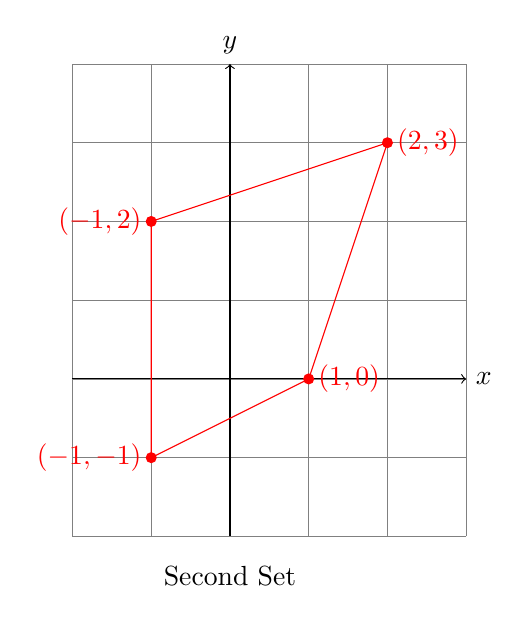
\begin{tikzpicture}[scale=1]
    % Grid and axes for second plot
    \draw[very thin,gray] (-2,-2) grid (3,4);
    \draw[->] (-2,0) -- (3,0) node[right] {$x$};
    \draw[->] (0,-2) -- (0,4) node[above] {$y$};
    
    % Points for second set
    \fill[red] (-1,2) circle (2pt) node[left] {$(-1,2)$};
    \fill[red] (2,3) circle (2pt) node[right] {$(2,3)$};
    \fill[red] (-1,-1) circle (2pt) node[left] {$(-1,-1)$};
    \fill[red] (1,0) circle (2pt) node[right] {$(1,0)$};
    
    % Draw convex hull
    \draw[red] (-1,2) -- (2,3) -- (1,0) -- (-1,-1) -- (-1,2);
    
    % Label
    \node at (0,-2.5) {Second Set};
\end{tikzpicture}
\end{center}

\pagebreak

\item\ \score{1}%8.
Fix an operator $\varphi : \RR^n \to \RR^n$.  If $X \subseteq \RR^n$
is convex and $\xx$ is an extreme point of~$X$, must $\varphi(\xx)$ be
an extreme point of~$\varphi(X)$?  What if $\varphi$ is assumed \red{Your counter example is wrong because the extreme points are in fact mapped to extreme points.}
invertible?
\\
\textbf{Solution}

For the first part, the answer is no.

\begin{align*}
  \begin{bmatrix}
    0 & 0\\
    0 & 1
  \end{bmatrix}
\end{align*}

You can see that the matrix is singular and collaspses the space to a line, so therefore the extreme points
are no longer extreme points after the transformation. For example, the square with vertices $(0,0)$, $(1,0)$, $(0,1)$, $(1,1)$,
the extreme points are $(0,0)$, $(1,1)$, $(0,1)$, $(1,0)$ but after the transformation the extreme points are $(0,0)$ and $(0,1)$.

For the second part, the answer is yes, because the transformation is invertible, therefore any line in the image can
be mapped back to a line in the original space, if a point is an extreme point in $X$, and not extreme in the image, \red{You need to be explicit about how this works.}
then it must be a convex combination of points in the output space, but since the transformation is invertible, you can take the inverse of
the line to show that the point itself couldn't have been an extreme point, contradicting the assumption.

\pagebreak

\item\ \score{2}%9.
Prove that the intersection of finitely many closed halfspaces
in~$\RR^n$ can have only finitely many extreme points.  Must it have
any extreme points at all? \magenta{ If it does have extreme points}, must the
intersection equal the convex hull of its extreme points?\rmagenta{You missed this.}

\textbf{Solution}

Claim \#1: Extreme points can only be on the boundary points of the intersection.

Proof: Assume for the sake of contradiction that there exists an extreme point $x$ that is not 
on the boundary of the intersection. Then $x$ has an open ball around it that is contained in the intersection. 
Then you can take two points in the open ball, and take a convex combination of the two points, which contains $x$,
contradicting the assumption that $x$ is an extreme point. Therefore all points are on the 
boundary, and the points on the boundary are points where the inequality of 
the halfspace space becomes equality.

Claim \#2: A point that satisfies less than $n$ restriction(satisfying restrictions means that the point is on the boundary of the halfspace) can't be an extreme point.

Take all the restrictions it does satisfy, then put them as a system of equations, and solve for a solution.
The null space of the matrix has dimension $>0$ because the point satisfies less than $n$ restrictions, and therefore
you can find a point in the null space $p$, and you can make $x+p$ and $x-p$, and these two points will also satisify
the restrictions, and their linear combinations will also satisfy the restrictions, as well.

  Ax=b,Where A is the set of restrictions, x is the point, and b is the vector of constants(the c values for the halfspaces).

\begin{align*}
  &rank(A)< n\\
  &\exists p \in N(A) \text{  N(\textit{A}) is the null space of A}\\
  &x+p \text{ and } x-p \text{ satisfy the restrictions}\\
  &\alpha (x+p) + (1-\alpha)(x-p) = x \text{ for } \alpha = 1/2
\end{align*}

Therefore the point is in between the two points, and therefore can't be an extreme point.

Claim \#3: A point that satisfies n or greater number of independent restrictions(meaning that the row vectors signifying the restrictions span the entire ambient space) is an extreme point.

Assume the point x satisfies n or greater number of restrictions, then the null space of the 
matrix is 0, now for the sake of contradiction assume that the point is not an extreme point, then there exists two points 
$y,z$ such that $x = \alpha y + (1-\alpha)z$. But the elements in the halfspaces when evaluated with
with linear funtional corresponding to the halfplane must have $\geq c$ for some constant.

But if you turn one of these $\geq (f(y)\geq c) $ into $>$, then you get $$ f(x) = c = \alpha f(y) + (1-\alpha)f(z) > f(x) = c$$, which is a contradiction, therefore 
the end points must also satisfy the restrictions, for all restrictions. But this implies that 
the points are also solutions to the matrix, which contradicts the fact that the matrix has a null space of 0.

Therefore the points satisfying n or greater number of restrictions are extreme points, and 
for any set of n restrictions there is only one point that satisfies all of them, and therefore
the number of restrictions is bounded by $\binom{total\;  number\; of\; restrictions}{n}$, which 
is finite, and therefore the number of extreme points is finite.

It is not necessariy that you have extreme points, if you have less restricitons than the ambient space, there are no extreme points
for example if you have 2 halfspces in $\RR^3$, and the intersection need not be equal to 
the convex hull, for example if you only have one extreme point, then the intersection isn't bounded.

\pagebreak

\item\ \score{3}%10.
Fix a column vector $\bb\in\RR^n$ and an $n \times n$ real matrix~$A$.
Show that the set of solutions $\{\xx \in \RR^n \mid A\xx \leq \bb\}$
of the inequality $A\xx \leq \bb$ is convex, where $\aa \leq \bb$ if
$a_i \leq b_i$ for all~$i$.  What kind of convex set is it?  (No need
to provide full justification of this last bit.)

\textbf{Solution}

Since you can write the inequality of each entry as a halfspace, and halfspaces are covex, then the 
intersection of the halfspaces is convex. The set is a polyhedron.

\pagebreak

\item\ \score{2}%11.
A \emph{cone} is a subset $C \subseteq \RR^n$ closed under nonnegative
scaling: $\xx \in C$ implies $\alpha \xx \in C$ for all $\alpha \in
\RR_{\geq 0}$.  A~ray $\RR_{\geq 0}\xx = \{\alpha\xx \mid \alpha \in
\RR_{\geq 0}\} \subseteq C$ is \emph{extreme} if $\xx \in \yy + C
\subseteq C$ implies $\yy \in \RR_{\geq 0}\xx$.  Let $\nu$ be an outer
support vector for a closed convex cone~$C$, so $\<\nu,\xx\> \leq 0$
for all $\xx \in C$.  Assume $\nu$ attains a unique maximum on~$C$.
% at the origin\/~$\0$.
Prove that the minimum angle between~$\nu$ and a unit vector~$\xx \in
C$ occurs when $\xx$ lies on an extreme~ray~of~$C$. \red{Your answer does not make use of the outer support vector condition.}

\textbf{Solution}

Claim \#1: A point that achieves the minimum angle can't be in the interior of the cone.

Assume that the point that achieves minimum angle is a point in the interioer.
Then there is an open ball around it, that is contained in the cone, where all the points in the 
open ball have a greater angle than the point, but this implies that the point is 
in the same direction as the $v$, because if you take that the plane that contains $v$ and the point,
the only way for the angle to increase by moving both clockwise and anti-clockwise, is if the angle between
them is 0.

Claim \#2: Points on the extreme ray, are not 'movable in all directions(don't have an open ball around them)'.

Take a point on the extreme ray, assume that there an open ball around it where all points are inside
the cone. Then take $y$ a point that is not a linear scaling of $x$.

\begin{align*}
  &\text{Let } N=x-y\\
  &x \in N + C\\
  &x = N + y, y \in C\\
\end{align*}

But since y isn't a linear scaling of x, that contradicts the definition of the extreme ray.
Therefore $x$ wasn't a point in the extreme ray, contradicting the assumption that you 
could make an ball around points on the extreme ray.


Since all points that have open balls around them can't achieve minimum angle, and only points on
the extreme ray don't have open balls, the unit vector $x$ has to be on an extreme ray, to achieve
minimum.

\pagebreak


\item\ \score{3}\label{kxn}%12.
How many $k \times n$ matrices of rank~$k$ with entries in a
field~$\FF_q$ of size~$q$ are there?  Hint: how many nonzero row
vectors are there in $\FF_q^n$?  How many vectors are linearly
independent from the first one?  How many are independent from the
first two?

\textbf{Solution}
There are $q^n-1$ valid row vectors, for the first one, because there are q options for each position
and excluding the zero vector, there are $q^n-1$ options.

For the second one you have $q^n-q$, because you can't include all the linear scaling of the first vector
which includes the zero, vector. 

For the $l$th row, you have $q^n - q^{l-1}$ options, because there are previously $l-1$ vectors
and you have to subtract all the linear combinatons from the set of possible vectors.

So the the total number of rank $k$ matrices is $\prod_{i=0}^{k-1} (q^n - q^i)$.

\pagebreak


\item\ \score{3}\label{free}%13.
Show that the action of~$\GL_k(F)$ on the set of $k \times n$ matrices
of rank~$k$ is \emph{free}: if $g \neq g'$ are invertible $k \times k$
matrices and $A$ is a $k \times n$ matrix of rank~$k$, then $gA \neq
g'A$.  Use this (and the previous exercise) to compute the cardinality
of the set $G_k(\FF_q^n)$ of $k$-planes in~$\FF_q^n$.  Hint: use
\#\ref{kxn} twice, once with $k = n$ and once with $k < n$.

\textbf{Solution}

Assume for the sake of contradiction that $gA=g'A$. The $gA-g'A=0$, but $g-g' \neq 0$ and $A\neq 0$
, but this implies that there is a non-zero row in $g-g'$ that is perpendicular to all 
the columns in $A$, but that implies all vectors are in the left null space of $A$
but the left null space of $A$ is 0, because the rank of $A$ is $k$, which is the entire output space.
So there can't be any elements to it, contradicting the fact that a nonzero vector is $g-g'$.

Since two different matrices in echelon form can't describe the same subspace, then the cardinality of
$G_k(\FF_q^n)$ is the same as the number of different echelon forms with dimension $k$. Given an echelon form you
can use $GL_k(F)$ actions to arrive at different matrices, that have the same column space, so 
the number of different $k$ planes is the number of distinct matrices divided by the number of 
number of matrices that describe the same subspace, which is the number of $k \times k$ invertible matrices.

So the cardinality is $\frac{ \prod_{i=0}^{k-1}(q^n-q^i) }{ \prod_{i=0}^{k-1}(q^k-q^i) }$.

\pagebreak

\item\ \score{3}%14.
Does the first claim in \#\ref{free} remain true if the rank of~$A$ is
less than~$k$?

\textbf{Solution}

No, because if the rank of $A$ is less than $k$, then there are non-zero vectors in the left null space of $A$.
For example what if $A=0$, then obviously $gA=g'A$ for all $g,g'$.
\pagebreak


\item\ \score{3}%15.
Use \#\ref{free} to count the number of Sets in the game of Set.
(Note: a Set is an affine line, not a linear subspace of
dimension~$1$, so this is not quite a special case of \#\ref{free}.
There is more than one way around this; I'll leave it to you to find
at least one.)  Confirm your count by counting a different way: a
line~$L$ is determined by any pair of points~on~$L$.

\textbf{Solution}

The number of one dimensional subspaces is $(3^4-1)/(3-1)=40$, therefore the number of lines 
that pass through the origin is 40, to get the total number of lines, move the starting around to all
points, and since each line intersects three points, you will triple count each point, so divide by 3,
so the total comes to $81 / 3 * 40 = 1080$.

Couting in a different way, a set is determined by any pair of points, the number of pair of points
is $81 \times 80 /2 = 3240$, and each line is counted by 3 different pairs, so you get $3240/3 = 1080 $.

\end{enumerate}


%%%%%%%%%%%%%%%%%%%%%%%%%%%%%%%%%%%%%%%%%%%%%%%%%%%%%%%%%%%%%%%%%%%%%%
\end{document}%%%%%%%%%%%%%%%%%%%%%%%%%%%%%%%%%%%%%%%%%%%%%%%%%%%%%%%%
%%%%%%%%%%%%%%%%%%%%%%%%%%%%%%%%%%%%%%%%%%%%%%%%%%%%%%%%%%%%%%%%%%%%%%


%%% Various Emacs customizations:
%%% Local Variables:
%%% fill-column: 70
%%% indent-tabs-mode: t
%%% TeX-electric-sub-and-superscript: nil
%%% TeX-brace-indent-level: 0
%%% LaTeX-indent-level: 0
%%% LaTeX-item-indent: 0
%%% TeX-master: t
%%% End